%%%%%%%% ICML 2026 SUBMISSION (blind) %%%%%%%%%%%%%%%%%%%%%%%%%%%%%%%%%%%%%%%%%%%%

\documentclass{article}

\usepackage{microtype}
\usepackage{graphicx}
\usepackage{subcaption}
\usepackage{booktabs}
\usepackage[T1]{fontenc}
\usepackage{hyperref}
\newcommand{\theHalgorithm}{\arabic{algorithm}}
\usepackage{icml2026}

\usepackage{amsmath}
\usepackage{amssymb}
\usepackage{mathtools}
\usepackage{amsthm}
\usepackage[capitalize,noabbrev]{cleveref}

\theoremstyle{plain}
\newtheorem{theorem}{Theorem}[section]
\newtheorem{proposition}[theorem]{Proposition}
\newtheorem{corollary}[theorem]{Corollary}
\theoremstyle{remark}
\newtheorem{remark}[theorem]{Remark}

% Results macros, filled in from the run logs
\newcommand{\REPSREAL}{300}
\newcommand{\REPSSYN}{500}
\newcommand{\TOTALTIME}{about 5 hours}

\icmltitlerunning{Shorter Prediction-Powered Intervals with Fixed Labels, Unlabeled Data and Predictor}

\begin{document}

\twocolumn[
  \icmltitle{Can Prediction-Powered Intervals Be Shorter With the Same Labels,\\
    Unlabeled Data and Predictor?}

  \icmlsetsymbol{equal}{*}

  \begin{icmlauthorlist}
    \icmlauthor{Anonymous Authors}{anon}
  \end{icmlauthorlist}

  \icmlaffiliation{anon}{Anonymous Institution}
  \icmlcorrespondingauthor{Anonymous Authors}{anonymous@example.com}

  \icmlkeywords{prediction-powered inference, semi-supervised inference, confidence intervals, efficiency, cross-fitting}

  \vskip 0.3in
]

\printAffiliationsAndNotice{}

\begin{abstract}
Prediction-powered inference (PPI) builds valid confidence intervals for a population mean from a small labeled sample, a large unlabeled sample, and a fixed predictor. We ask whether the existing intervals can be made shorter when the labeled set, the unlabeled set, and the predictor are all held fixed, with nominal coverage still required. We show that the answer is governed by one quantity, the nonlinear share $\kappa$ of the calibration function $m(Z)=\mathbb E[Y\mid Z]$ beyond its best linear fit. For this estimator class, the asymptotic variance of any cross-fitted calibrated estimator equals the efficient bound plus $(1-a)\mathrm{Var}(\hat m-m)/n$, where $a=n/(n+N)$. PPI++ therefore attains the bound exactly when $m$ is affine in the information used, and a nonlinear calibrator helps only when its error is smaller than the linear misfit. In simulations with known truth, a cross-fitted spline calibrator shortens intervals by $17$--$19\%$ when calibration is strongly nonlinear (the efficient bound is $24\%$), and it widens them by $1$--$16\%$ when it is not. On seven public pools with exact coverage checks, the estimated nonlinear share is at most $5\%$; the flexible estimator is $5$--$11\%$ wider at $n=50$, $1$--$4\%$ wider at $n=200$, and within $1\%$ of PPI++ at $n=1000$, while all methods cover at the nominal level up to small-sample effects. Shorter intervals in this setting are available only when calibration is materially nonlinear and the labeled sample is large enough to learn it.
\end{abstract}

\section{Introduction}
\label{sec:intro}

Many scientific analyses share one bottleneck. Gold-standard labels are expensive, a much larger set of covariates is cheap, and a pretrained predictor can be run on every unit. Examples are remote-sensing land-cover classes, galaxy morphology, and census-based income or insurance indicators. The analyst wants a confidence interval for a population quantity such as a mean or prevalence, with guaranteed coverage and as little width as possible.

Prediction-powered inference (PPI) answers this with a rectifier: average the predictor over the unlabeled sample and add the labeled residual correction \citep{angelopoulos2023ppi}. PPI++ replaces the fixed correction with a data-driven weight \citep{angelopoulos2023ppiplus}, and cross-fitting handles predictors trained on the labels \citep{zrnic2023cross}. These methods all hold the data-collection design fixed in one respect: they accept the labeled set, the unlabeled set, and the predictor as given. Our question is what is left to gain under exactly that constraint. Holding labels, unlabeled covariates, and the predictor fixed, can the existing intervals be shortened without weakening coverage? If so, by how much, and under what conditions does the answer change?

We make three contributions.

\textbf{(1) An exact gap.} For the estimator class in which the mean is corrected by a calibrator $\hat m$ fitted on labeled data, the asymptotic variance is $V^\star+(1-a)\mathrm{Var}(\hat m-m)/n$, where $V^\star$ is the efficient bound for the information used, $m$ is the conditional mean, and $a=n/(n+N)$ is the labeled fraction (\cref{prop:var,thm:bound}). PPI++ equals the bound plus $(1-a)\Delta_L/n$, where $\Delta_L$ is the squared misfit of the best linear calibrator. PPI++ is therefore not efficient exactly when $m$ is nonlinear in the information used (\cref{cor:when}). The same argument shows that covariates beyond the predictor help through the same term (\cref{cor:cov}).

\textbf{(2) A practical condition.} A flexible calibrator helps only when its error variance is below the linear misfit, $\mathrm{Var}(\hat m-m)<\Delta_L$ (\cref{cor:learned}). This is a testable statement about the labeled sample, and it implies that flexibility can backfire at small $n$.

\textbf{(3) Evidence on known-truth and real data.} Using cross-fitting, the estimator stays exactly unbiased for any learner (\cref{prop:unbiased}). On synthetic problems, a spline calibrator shortens intervals by 17--19\% when calibration is strongly nonlinear, against an efficient-bound reduction of 24\%. It widens them when calibration is linear, by up to 16\% at $n=50$. On seven public pools with exact coverage checks, the estimated nonlinear share is at most 5\% of the linear residual variance, so there is little to gain. The flexible estimator is 5--11\% wider at $n=50$, 1--4\% wider at $n=200$, and within 1\% of PPI++ by $n=1000$. Coverage is at the nominal level for all methods, except for expected small-sample undercoverage on heavy-tailed incomes.

The answer is therefore conditional. The interval can be shortened with the same data and predictor only when the calibration function is materially nonlinear and the labeled sample is large enough to learn it. On the public pools we could check, the gain is not available at the sample sizes that matter most in practice. We state the conditions precisely, give the formulas to check them, and report the failures.


\section{Related Work}
\label{sec:related}

\paragraph{Prediction-powered inference.}
\citet{angelopoulos2023ppi} introduced prediction-powered inference (PPI): a small labeled sample is combined with a large unlabeled sample and the output of a fixed machine-learning predictor, and the rectifier $\bar Y_L-\bar f_L$ corrects the bias of the predictor, giving valid intervals for means, quantiles, and regression coefficients without assumptions on the predictor. \citet{angelopoulos2023ppiplus} (PPI++) add a data-driven tuning parameter $\lambda$ that interpolates between using only labels and using the predictor at full strength, and show that the resulting intervals never widen relative to labeled-only intervals in the cases they study. Our PPI++ baseline is the optimal linear calibration within this family. \citet{zrnic2023cross} cross-fit the predictor when it is trained on the same labels, and \citet{zrnic2024active} choose which points to label. Both change the sampling or fitting setting, which we hold fixed. \citet{fisch2024strat} stratify on the predictor output, and we compare to their point estimator directly (Section~\ref{sec:exp}).

\paragraph{Semiparametric efficiency with missing outcomes.}
Our efficiency bound is the standard one for estimating a mean when outcomes are missing at random with known probability, and the augmented estimator that attains it is classical \citep{robins1994estimation,tsiatis2006semiparametric}. Double/debiased machine learning \citep{chernozhukov2016dml} uses cross-fitting with a learned nuisance function to get valid inference under flexible fitting. The setting here is simpler, because the only nuisance is $m(Z)=\mathbb E[Y\mid Z]$ and it enters the estimator linearly, which lets us state the variance exactly (Proposition~\ref{prop:var}). General theory of semi-supervised mean estimation with unlabeled covariates is developed in \citet{zhang2019semi}, and semi-supervised linear regression in \citet{chakrabortty2018efficient}; we did not rely on their efficiency statements beyond the setting they describe.

\paragraph{What this paper adds.}
The question we address is narrower than the PPI literature: holding the labeled set, the unlabeled set, and the predictor fixed, can the existing intervals be made shorter without any new data or assumptions beyond validity? We answer with an explicit gap formula (Theorem~\ref{thm:bound}), a condition under which a learned calibrator helps (Corollary~\ref{cor:learned}), and a practical cross-fitted estimator whose gains we measure on real and synthetic data.


\section{Setting, Estimators, and Efficiency}
\label{sec:setting}

\paragraph{Sampling model.}
We observe $n$ labeled units $(Z_i,Y_i)$ and $N$ unlabeled units $\tilde Z_j$, where $Z=(f(X),\,\cdot)$ collects the information available to the analyst (the prediction alone, or the prediction together with covariates $X$). All units are i.i.d. from one population, and labeled and unlabeled samples are independent. Let $a=n/(n+N)$ denote the labeled fraction and $\theta=\mathbb E[Y]$ the target (a mean, including prevalence for binary $Y$). Write $m(Z)=\mathbb E[Y\mid Z]$, $\sigma^2(Z)=\mathrm{Var}(Y\mid Z)$, and let $L(Z)$ be the best linear predictor of $Y$ from $Z$ (with intercept).

\paragraph{A common form.}
For any calibrator $\hat m$ (a function fitted on labeled data), define
\begin{equation}
\hat\theta_{\hat m}
=\bar Y_L+(1-a)\Big(\bar{\hat m}_U-\bar{\hat m}_L\Big)
=\underbrace{\bar Y_L-(1-a)\bar{\hat m}_L}_{\text{labeled}}
+\underbrace{(1-a)\bar{\hat m}_U}_{\text{unlabeled}}\,,
\label{eq:common}
\end{equation}
where $\bar{\hat m}_L$ and $\bar{\hat m}_U$ are sample means over labeled and unlabeled units. Equivalently, $\hat\theta$ is the average of $\hat m$ over the pooled sample plus the labeled residual correction $\bar Y_L-\bar{\hat m}_L$. Taking $\hat m=f$ and $\hat m$ linear gives PPI and PPI++ (with $\lambda=(1-a)\beta$, $\beta=\mathrm{Cov}(Y,f)/\mathrm{Var}(f)$, which is the PPI++ value $\lambda^\star=\mathrm{Cov}(Y,f)/\{\mathrm{Var}(f)(1+n/N)\}$).

\paragraph{Cross-fitted calibrator.}
Split the labeled units into $K$ folds. Fit $\hat m_{-k}$ on the labeled units outside fold $k$. For labeled unit $i$ in fold $k(i)$ set $\hat m_L(Z_i)=\hat m_{-k(i)}(Z_i)$ (out-of-fold), and for unlabeled units set $\hat m_U(\tilde Z_j)=K^{-1}\sum_k\hat m_{-k}(\tilde Z_j)$. The estimator is \eqref{eq:common} with these values, and the variance estimate is
\begin{equation}
\widehat V=\frac{\widehat{\mathrm{Var}}_L\{Y-(1-a)\hat m_L\}}{n}+\frac{(1-a)^2\,\widehat{\mathrm{Var}}_U(\hat m_U)}{N}\,,
\qquad \mathrm{CI}=\hat\theta\pm z_{1-\alpha/2}\sqrt{\widehat V}.
\label{eq:cfvar}
\end{equation}
With $\hat m=L$ fitted on all labeled data, \eqref{eq:cfvar} reduces to the PPI++ variance formula.

\subsection{Three facts about this estimator class}

\begin{proposition}[Exact unbiasedness under cross-fitting]
\label{prop:unbiased}
If the fold fits are exchangeable (e.g., random folds and a deterministic learner) and integrable, then $\mathbb E\,\hat\theta=\theta$ for every $n$ and $N$, whatever the learner is and however large its error.
\end{proposition}
\begin{proof}[Proof sketch]
$\mathbb E\bar Y_L=\theta$. Each out-of-fold value has the same mean $\mu_{\hat m}=\mathbb E\hat m_{-k}(Z)$ by exchangeability, so $\mathbb E\bar{\hat m}_L=\mathbb E\bar{\hat m}_U=\mu_{\hat m}$, and the correction term has mean zero.
\end{proof}

Unbiasedness does not depend on the learner, which is why cross-fitting matters here. Without it, $\hat m_L$ and $Y_L$ share data and the labeled residual term carries an in-sample bias.

\begin{proposition}[Asymptotic variance]
\label{prop:var}
Suppose the fold fits converge in $L_2$ to a fixed function $\tilde m$ (possibly $\neq m$), with finite fourth moments of $Y$ and $\tilde m$. Then $\sqrt n(\hat\theta-\theta)\Rightarrow\mathcal N(0,V(\tilde m))$, where
\begin{equation}
n\,V(\tilde m)=\mathbb E[\sigma^2(Z)]+a\,\mathrm{Var}\{m(Z)\}+(1-a)\,\mathrm{Var}\{\tilde m(Z)-m(Z)\}.
\label{eq:Vcal}
\end{equation}
\end{proposition}
\begin{proof}[Proof sketch]
Write $\delta=\tilde m-m$. Linearizing \eqref{eq:common} gives $\hat\theta-\theta\approx(\bar Y_L-\theta)-(1-a)(\bar{\tilde m}_L-\mu)+(1-a)(\bar{\tilde m}_U-\mu)$. The labeled and unlabeled pieces are independent, so $V=\mathrm{Var}\{Y-(1-a)\tilde m\}/n+(1-a)^2\mathrm{Var}(\tilde m)/N$. Since $Y-(1-a)\tilde m=e+am-(1-a)\delta$ with $e=Y-m$ uncorrelated with any function of $Z$, expanding and using $(1-a)^2/N=a(1-a)/n$, the coefficient of $\mathrm{Var}(m)$ is $a^2+a(1-a)=a$, that of $\mathrm{Cov}(m,\delta)$ is $-2a(1-a)+2a(1-a)=0$, and that of $\mathrm{Var}(\delta)$ is $(1-a)^2+a(1-a)=1-a$, which gives \eqref{eq:Vcal}.
\end{proof}

Two consequences matter. First, the calibrator's \emph{error} enters the variance only through $\mathrm{Var}(\tilde m-m)$, with no bias term. Second, the penalty carries the factor $1-a=N/(n+N)$, so it vanishes when $N=0$.

\begin{theorem}[Efficiency bound and the PPI++ gap]
\label{thm:bound}
Let $\mathcal M_Z$ be the model in which $Z$ is the only information used, $(Z,Y)$ is otherwise unrestricted, and labels are missing completely at random with probability $a$. The semiparametric efficiency bound for $\theta$ is
\begin{equation}
V^\star(Z)=\frac{\mathbb E[\sigma^2(Z)]+a\,\mathrm{Var}\{m(Z)\}}{n},
\label{eq:bound}
\end{equation}
attained by \eqref{eq:common} with $\tilde m=m$. Let $\Delta_L=\mathbb E\{m(Z)-L(Z)\}^2$. Then the PPI++ estimator (linear $\hat m$ in $Z$) has
\begin{equation}
V_{\mathrm{PPI}\text{++}}-V^\star(Z)=\frac{(1-a)\,\Delta_L}{n}.
\label{eq:gap}
\end{equation}
\end{theorem}
\begin{proof}[Proof sketch]
For the observation $O=(R,RY,Z)$ with $R\sim\mathrm{Bernoulli}(a)$ independent of $(Z,Y)$, the efficient influence function under missing-at-random outcomes is $\psi=\frac{R}{a}\{Y-m(Z)\}+m(Z)-\theta$ (Robins, Rotnitzky and Zhao, 1994; Tsiatis, 2006). Its variance per unit is $\mathbb E\sigma^2/a+\mathrm{Var}(m)$, and with $n+N$ units and $a(n+N)=n$ this gives \eqref{eq:bound}. For PPI++, $\tilde m=L$, so $\delta=L-m$ has mean zero and $\mathrm{Var}(\delta)=\Delta_L$; apply Proposition~\ref{prop:var}.
\end{proof}

\begin{corollary}[When can the interval shrink?]
\label{cor:when}
Write $\rho=V^\star/V_{\mathrm{PPI}\text{++}}$. The asymptotic CI width ratio of the efficient interval to PPI++ is $\sqrt\rho$, where
\[
1-\rho=\frac{(1-a)\,\Delta_L}{\mathbb E(Y-L)^2+a\,\mathrm{Var}(L)}.
\]
Hence: (i) PPI++ is efficient for the information $Z$ iff $m(Z)$ is affine in $Z$ ($\Delta_L=0$); (ii) if $N=0$ there is no gain; (iii) as $a\to0$ the gain tends to $\Delta_L/\mathbb E(Y-L)^2$, the share of the linear calibrator's residual variance explained by the nonlinear part of $m$.
\end{corollary}

\begin{corollary}[Covariates beyond the prediction]
\label{cor:cov}
Let $Z^+=(f,X)$ and $Z=f$. Then $V^\star(Z)-V^\star(Z^+)=\frac{(1-a)}{n}\mathbb E\{m(Z^+)-m(Z)\}^2$. Using covariates helps by exactly the same type of term as nonlinear calibration.
\end{corollary}

\begin{corollary}[Learned calibrators]
\label{cor:learned}
Let $\hat m$ converge to $\tilde m$. The cross-fitted estimator beats PPI++ asymptotically iff
\[
\mathrm{Var}(\tilde m-m)<\Delta_L,
\]
i.e., the calibrator's error must be smaller than the linear calibrator's misfit. The asymptotic width ratio is $\sqrt{1+(1-a)\{\mathrm{Var}(\tilde m-m)-\Delta_L\}/(nV_{\mathrm{PPI}\text{++}})}$.
\end{corollary}

These statements are asymptotic and conditional on the chosen information set. They do not say that a valid interval can never be shorter than PPI++ under other assumptions, for example bounded outcomes or exact small-sample constructions. The claim is about regular Wald-type intervals built from the same $(Z_L,Y_L,Z_U)$.


\section{Experimental Design}
\label{sec:exp}

\paragraph{Target and methods.}
The target is the population mean $\mathbb E[Y]$. For every method we report a Wald interval at nominal 95\% level, $\hat\theta\pm1.96\sqrt{\widehat V}$, and compare to:
(i) \emph{classical}, the labeled-only mean;
(ii) \emph{PPI} with $\lambda=1$;
(iii) \emph{PPI++} with the plug-in optimal $\lambda$ (linear calibration on $f$; or on $(f,X)$ when covariates are used);
(iv) \emph{stratified PPI} (Fisch et al., 2024, $\lambda_k=1$), with quantile strata of $f$ and unlabeled-estimated stratum weights, using the linearized variance;
(v) \emph{cross-fitted calibration} (ours), with 5-fold cross-fitting and three learners: a cubic B-spline ridge model (primary), gradient boosting, and linear regression.
The primary learner was chosen before the main runs using development seeds disjoint from the reported ones. The rule was the lowest mean width ratio to PPI++ across the five synthetic scenarios, subject to nominal coverage. The spline calibrator won on average (0.967, versus 0.978 for boosting and 1.009 for linear), and boosting was marginally better only in the nonlinear scenario. We report all learners on the real data.

\paragraph{Real data.}
We use the nine pools distributed with \texttt{ppi-python} v0.2.3\footnote{\url{https://github.com/aangelopoulos/ppi_py}}, which contain labels and predictions for every unit. Seven pools give exact coverage checks: \texttt{galaxies}, \texttt{forest}, \texttt{gene\_expression}, \texttt{alphafold}, \texttt{census\_income}, \texttt{census\_healthcare}, and \texttt{census\_education}. Pools \texttt{plankton} and \texttt{ballots} have no labels on part of the unlabeled pool, so their target is undefined and we exclude them from coverage (a shift problem for \texttt{plankton}). Covariates are used only in the \emph{fX} regime; constant columns are dropped. Each pool is treated as the finite population. Labeled and unlabeled samples are drawn i.i.d.\ with replacement from it, so the sampling model is exactly the i.i.d.\ model of Section~\ref{sec:setting} and the target is the pool mean. Sample sizes are $n\in\{50,100,200,500,1000\}$ with $N/n\in\{1,4,16\}$. We use \REPSREAL{} replications per cell.

\paragraph{Synthetic data.}
Five data-generating processes have known $\mathbb E[Y]$ (Monte Carlo truth with $10^7$ draws). \emph{linear} has $m$ affine in $f$, so PPI++ should be efficient. \emph{nonlinear} has $m(f)=\sin(2f)+f/2$. \emph{binary} has a Bernoulli outcome and a miscalibrated probability predictor. \emph{xonly} has $m$ depending on a covariate not in $f$. \emph{heavy} is nonlinear with $t_3$ noise. We use \REPSSYN{} replications per cell over the same grid.

\paragraph{Theory checks.}
To test Propositions~\ref{prop:var} and Corollary~\ref{cor:when} without learner noise, we run oracle calibrators $\hat m=m+s\,h(f)$, where $h$ is a centred, unit-variance function and $s\in\{0,0.1,0.2,0.4\}$ gives $\mathrm{Var}(\hat m-m)=s^2$. Population constants come from one large draw.

\paragraph{Reproducibility.}
Seeds are fixed per cell and derived from the cell's indices, so every number in the paper is regenerated by \texttt{run\_main.sh}. Compute ran on a 4-CPU quota; the full pipeline took \TOTALTIME{}.


\section{Results}
\label{sec:results}

All intervals are nominal 95\% Wald intervals. Coverage is reported with Monte Carlo standard errors of about $0.01$ at $R=\REPSSYN$ and $0.013$ at $R=\REPSREAL$. Width ratios are relative to PPI++ on the same replications, with the same labeled and unlabeled samples. The efficient bound is the asymptotic width ratio of the oracle calibrator for the information used (for \emph{f}-only pools it is $\sqrt{V^\star(f)/V_{\rm PPI++}}$, and for pools with covariates the same with $(f,X)$ against PPI++ with linear covariate adjustment).

\subsection{Synthetic data with known truth}

\cref{fig:synth} plots the width ratio against labeled size $n$ at $N=4n$. Each panel is one scenario. Under \emph{linear calibration}, $m$ is affine in $f$, and the bound is 1: no method beats PPI++, and the flexible calibrators widen intervals by $16\%$ at $n=50$ (spline) and $19\%$ (boosting), shrinking to $1\%$ at $n=1000$. This is the predicted cost $(1-a)\mathrm{Var}(\hat m-m)/n$ with $\hat m$ estimated from few labels.

Under \emph{nonlinear calibration}, the spline calibrator gives width ratios $0.83$, $0.81$ and $0.82$ at $n=50,200,1000$, against a bound of $0.756$. The gap to the bound is the learner's own error, which is consistent with the theory: the realized gain is the bound's gain minus $(1-a)\mathrm{Var}(\hat m-m)/n$. Boosting is slightly better at $n\ge200$ ($0.77$--$0.80$) and also narrower at $n=50$ ($0.86$). The stratified PPI estimator of \citet{fisch2024strat} does not gain in this scenario (ratio $0.99$--$1.00$); its piecewise-constant calibrator has a larger error than the spline. \emph{Binary} outcomes give a small bound (0.98) and small gains at $n\ge200$. \emph{Covariates beyond $f$} make PPI++ on $f$ alone inefficient through $E(m_X-m_f)^2$: the spline with covariates reaches $0.82$ against a bound of $0.76$. \emph{Heavy-tailed} noise gives 0.88--0.90 against a bound of 0.86, with coverage unaffected.

Coverage is between $0.92$ and $0.97$ for PPI, PPI++ and the cross-fitted estimators in every cell, with no systematic difference between them. Stratified PPI is the exception: its coverage falls to $0.91$ in several small-sample cells (for example, $n=50$ with $N=4n$ under the binary and heavy-tailed scenarios), where the estimated stratum weights and small per-stratum samples make the linearized variance too small.

\begin{figure*}[t]
  \centering
  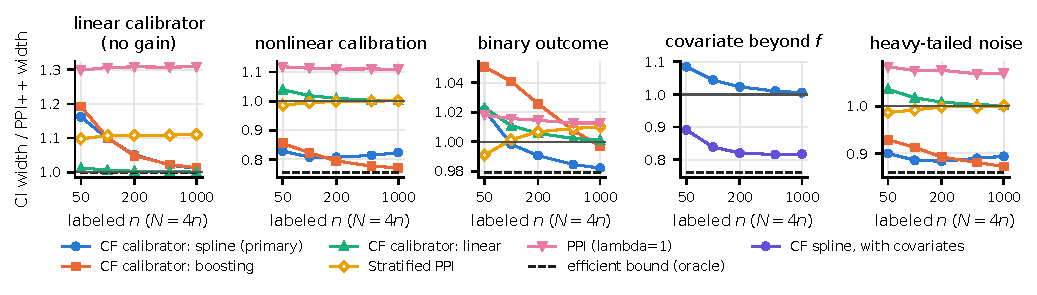
\includegraphics[width=\textwidth]{figures/fig_synth.pdf}
  \caption{Synthetic data, $N=4n$, 500 replications per point. The vertical axis is the mean CI width relative to PPI++ on the same samples. Dashed: efficient bound for the information used (oracle calibrator). Points above 1 are wider than PPI++.}
  \label{fig:synth}
\end{figure*}

\subsection{Agreement with the variance formulas}

To test the formulas without learner noise, \cref{tab:theory} (appendix) compares Monte Carlo standard deviations and width ratios with the predictions of \cref{prop:var} for oracle calibrators with error variance $s^2\in\{0,0.04\}$ and $\{0,0.16\}$. Across the five scenarios, three values of $\mathrm{Var}(\hat m-m)$, $n\in\{50,200,1000\}$ and $N/n\in\{1,4,16\}$, the width ratios agree with the prediction to within $2\%$ (largest discrepancy $1.7\%$, nonlinear scenario), and the Monte Carlo standard deviations agree to within $1\%$ (median) except one case: the heavy-tailed scenario at $n=1000$, where the predicted SD is $9\%$ too small. We attribute this to the slow convergence of the Monte Carlo estimate of the population variance of $t_3$ noise (its fourth moment is infinite); we did not verify this directly. These checks hold for the bound itself (e.g., $0.757$ observed against $0.756$ predicted in the nonlinear case).

\subsection{Public pools with exact coverage checks}

We use the seven pools that have labels and predictions for every unit (\cref{sec:exp}). \cref{tab:real} reports, for each pool and information set, the efficient-bound ratio at $N=4n$ (computed from the pool-level constants with the formula in \cref{cor:when}) and the realized width ratio of the spline calibrator at $n=50,200,1000$. \cref{fig:real} shows the realized ratios at $n=200$ for all calibrators.

The bound is between $0.98$ and $1.00$ for every pool and information set. The estimated nonlinear shares $\kappa=\Delta_L/\mathbb E(Y-L)^2$ are $0.2\%$ to $5.4\%$ (\cref{tab:pool}, appendix). Forest, alphafold and gene expression have the largest shares and the largest possible gains. Realized gains are absent. At $n=50$ the spline calibrator is $5$--$11\%$ wider than PPI++; at $n=200$ it is $1$--$4\%$ wider; at $n=1000$ it is within $1\%$. The boosting calibrator is wider still ($2$--$9\%$ at $n=200$), and the linear calibrator is within $2\%$ of PPI++ at $n=200$. Adding covariates to PPI++ changes width by less than $1\%$ at $n\ge200$ on these pools.

PPI++ itself does shorten intervals substantially relative to the labeled-only mean: classical intervals are $1.14$--$1.98$ times wider than PPI++ at every $n$ we tried (\cref{tab:realsens} reports $n=200$). The pools therefore confirm the value of prediction-powered inference, but not of further flexibility.

Coverage at the nominal level holds for all methods on all pools. Per-cell coverage is between $0.89$ and $0.98$ for $n\ge200$, with the lowest values on census income. At $n=50$, census income undercovers for every method, PPI++ and the classical mean included: coverage is $0.83$--$0.89$. The heavy right tail of the income outcome makes the normal approximation poor at this size. Forest at $n=50$ over-covers ($0.96$--$0.97$) because the outcome is discrete.

\begin{table*}[t]
  \centering
  \caption{Public pools (exact coverage checks, $N=4n$, \REPSREAL{} replications per cell). \emph{Bound}: efficient-bound width ratio vs PPI++ at $a=1/5$, from pool-level quantities. $n=50,200,1000$: realized width ratio of the spline-calibrated estimator vs PPI++ (with linear covariate adjustment in the $f{+}X$ rows). Coverage columns give the range over all $(n,N/n)$ cells.}
  \label{tab:real}
  \small
  \begin{tabular}{llcccccc}
\toprule
Pool & Info & Bound & $n{=}50$ & $n{=}200$ & $n{=}1000$ & CF cov.\ range & Baseline cov.\ range \\
\midrule
galaxies & f & 0.997 & 1.051 & 1.015 & 1.004 & 0.927--0.963 & 0.923--0.960 \\
forest & f & 0.980 & 1.072 & 1.015 & 1.000 & 0.910--0.970 & 0.913--0.963 \\
gene expr. & f & 0.997 & 1.080 & 1.014 & 1.002 & 0.933--0.973 & 0.927--0.970 \\
alphafold & f & 0.992 & 1.067 & 1.015 & 1.002 & 0.913--0.957 & 0.903--0.963 \\
alphafold & f+X & 0.987 & 1.092 & 1.021 & 1.003 & 0.923--0.967 & 0.897--0.963 \\
census income & f & 0.998 & 1.095 & 1.034 & 1.007 & 0.840--0.953 & 0.833--0.947 \\
census income & f+X & 0.995 & 1.107 & 1.039 & 1.007 & 0.830--0.953 & 0.820--0.957 \\
census health & f & 0.999 & 1.047 & 1.014 & 1.003 & 0.940--0.977 & 0.930--0.970 \\
census health & f+X & 0.999 & 1.053 & 1.015 & 1.004 & 0.917--0.967 & 0.920--0.957 \\
census educ. & f & 0.999 & 1.067 & 1.021 & 1.004 & 0.927--0.973 & 0.910--0.967 \\
census educ. & f+X & 0.998 & 1.105 & 1.035 & 1.008 & 0.917--0.960 & 0.903--0.953 \\
\bottomrule
\end{tabular}

\end{table*}

\begin{figure}[t]
  \centering
  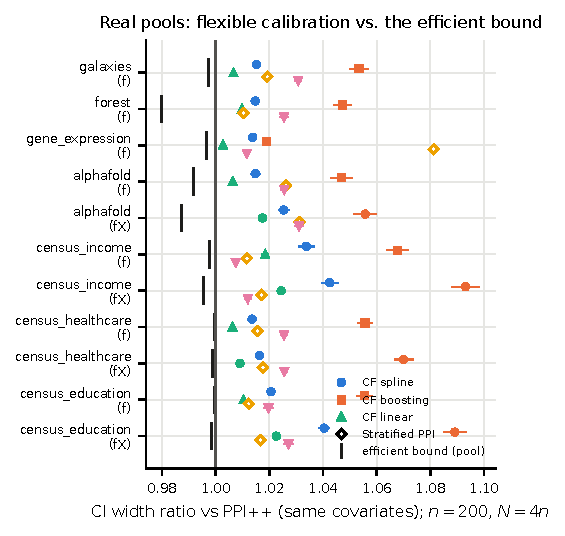
\includegraphics[width=\columnwidth]{figures/fig_real.pdf}
  \caption{Real pools at $n=200$, $N=4n$. Points: realized width ratios vs PPI++ (with covariate adjustment in $f{+}X$ rows) for each calibrator, with 95\% Monte Carlo intervals. Ticks: efficient bound from pool-level quantities.}
  \label{fig:real}
\end{figure}

\subsection{Larger labeled samples}

To test whether the realized gap closes with more labels, we extended four pools that span the range of nonlinear shares to $n=5{,}000$ and $n=20{,}000$ ($N=4n$, 100 replications per cell). The spline calibrator's width ratio moves down toward the bound as $n$ grows: at $n=20{,}000$ it is $0.995$ on \texttt{forest} (bound $0.980$), $0.998$ on \texttt{gene\_expression} (bound $0.997$), $0.998$ on \texttt{alphafold} (bound $0.992$), and $1.000$ on \texttt{census\_education} with covariates (bound $0.998$). Realized gains therefore appear only at the largest sample sizes, and on \texttt{forest} they recover a quarter of the bound's $2\%$. Coverage stays between $0.92$ and $0.96$ for PPI++ and the spline calibrator (100 replications, Monte Carlo standard error about $0.025$).

\subsection{Summary of conditions}

Across the three evidence sources, the width reduction is governed by two quantities that can be estimated from the data at hand: the nonlinear share $\kappa$ of the calibration function (which sets the bound), and the learner's error variance at the available $n$ (which sets the realized gain). A reduction is realized when $\mathrm{Var}(\hat m-m)<\Delta_L$ and only then. Under linear calibration, under small $n$ relative to the complexity of $m$, or under small nonlinear share, PPI++ is the better interval.


\section{Discussion and Limitations}
\label{sec:discussion}

\paragraph{When the interval can be shortened.}
Holding the labeled set, the unlabeled set, and the predictor fixed, a shorter valid interval requires three things at once: the calibration function $m$ must be nonlinear in the information used, the nonlinear part must be material compared with the linear residual variance ($\kappa$ large), and the labeled sample must be large enough that a flexible calibrator's error is smaller than that nonlinear part. The first two are properties of the problem; the third depends on $n$. Our simulations reach the bound up to the learner's error. The public pools satisfy the first condition only weakly: their nonlinear shares are at most $5\%$, which bounds the available gain at roughly $2\%$ of the interval width at $N=4n$.

\paragraph{Practical recipe.}
We recommend the following. (i) Fit a linear calibrator and compute $\kappa$ on the labeled data with cross-fitting; if it is small, report PPI++ and stop. (ii) If $\kappa$ is large, fit a smooth calibrator with cross-fitting and check whether its out-of-fold error is below $\Delta_L$; if it is not, the linear interval is the better choice. (iii) Report the chosen estimator and its alternatives, since the choice is data-dependent. The formulas in Theorem~\ref{thm:bound} and Corollary~\ref{cor:learned} give the bound and the break-even condition, and both are computable from the labeled sample.

\paragraph{Why more flexibility can hurt.}
Cross-fitting protects validity: the estimator stays unbiased for any learner. It does not protect width. A learner adds $(1-a)\mathrm{Var}(\hat m-m)/n$ to the variance, which is the reason a spline calibrator widens intervals by $16\%$ when $m$ is linear and $n=50$. Boosting, which has more variance at small $n$, widens them by $19\%$. In practice, a cross-validated choice between linear and flexible calibrators would reduce this cost, but it adds a selection step whose effect on coverage we did not study.

\paragraph{Comparison with stratification.}
Stratified PPI \citep{fisch2024strat} uses a piecewise-constant calibrator on the predictor. In our experiments it did not gain over PPI++ in any scenario, and it was $1$--$8\%$ wider on the real pools. We note a point that matters for implementation: when strata weights are estimated from the unlabeled data, as is standard, the variance must include the between-stratum term $\mathrm{Var}_U(f+\bar r_{b(f)})$. Treating the weights as known, as the variance formula in that paper does, undercovers in our development runs (coverage 0.86 across development cells, and a width ratio of about 0.67 on the linear scenario). The corrected linearization is the one used in this paper.

\paragraph{Limitations.}
\begin{itemize}
  \item \emph{Asymptotic statements.} Propositions~\ref{prop:var} and Theorem~\ref{thm:bound} are first-order. The variance formula is a Wald approximation; at $n=50$ with heavy-tailed or discrete outcomes it undercovers (census income) or over-covers (forest). Exact or bounded-outcome intervals could be tighter at small $n$; we did not evaluate them.
  \item \emph{Mean target and i.i.d. sampling.} We study $\mathbb E[Y]$, which includes prevalence. Quantiles, regression coefficients, and covariate or label shift are not covered. The real-data target is the pool mean, and the pools are treated as populations with i.i.d.\ resampling.
  \item \emph{Real data coverage.} Only seven pools had full labels and predictions. \texttt{plankton} has labels on a different year than its unlabeled set, which is a distribution-shift problem outside our question, and \texttt{ballots} has no labels on its unlabeled pool, so coverage is undefined. We did not run folktables or other external datasets.
  \item \emph{Estimated bound.} The pool-level bound uses a cross-fitted gradient-boosting estimate of $m$. For some pools that estimate is less accurate than the linear fit, so the reported bound is conservative: $\Delta_L$ is inflated by estimation error. The bound columns are therefore an upper estimate of the available gain.
  \item \emph{Learner choice.} The spline calibrator was selected on synthetic development data. Other learners could do better on particular real pools; Table~\ref{tab:realsens} reports all three we tried.
  \item \emph{Sample size.} Our main grid goes to $n=1000$; on four pools we also ran $n=5{,}000$ and $20{,}000$ (\cref{sec:results}). The realized gain approaches the bound only slowly: on \texttt{forest} at $n=20{,}000$ it is half a percent against a bound of two percent. Larger labeled samples than we could check may be needed before the flexible estimator reaches the bound on pools with small $\kappa$.
\end{itemize}

\paragraph{Scope of the claim.}
The result concerns regular Wald-type intervals that use the same $(Z_L,Y_L,Z_U)$. It does not rule out shorter intervals from different assumptions, such as bounded outcomes or additional unlabeled covariates beyond those we used. Within the stated information set, the efficient bound is a lower bound on asymptotic variance for regular estimators.


\section*{Impact Statement}
This paper studies how to report uncertainty more tightly for population means estimated from machine-learning predictions, and it shows when the tightening is not available. Shorter intervals can help when labels are expensive, but they rely on the stated assumptions (i.i.d. sampling and a fixed predictor). The paper reports where those assumptions are likely to fail, including covariate shift, and it does not claim validity under them. We do not foresee direct negative societal consequences beyond those of the underlying applications.

\bibliography{refs}
\bibliographystyle{icml2026}

\newpage
\appendix
\onecolumn

\section{Proofs}
\label{app:proofs}

We write $\mu=\mathbb E[Y]$, $e=Y-m(Z)$, $\sigma^2(Z)=\mathbb E[e^2\mid Z]$, and $a=n/(n+N)$, with $n,N\to\infty$ and $N/n$ bounded away from zero, so that $a\in(0,1]$ is fixed.

\paragraph{Proposition 1 (unbiasedness).}
Let the labeled sample be split into $K$ folds at random, and let the learner be applied to the $K-1$ other folds. Out-of-fold values $\hat m_L(Z_i)$ and fold-averaged values $\hat m_U(\tilde Z_j)$ are evaluated at points independent of the fit, so each has expectation $\mu_{\hat m}=\mathbb E\,\hat m_{-k}(Z)$ (the fold models are exchangeable under random folds). Then
\[
\mathbb E\hat\theta=\mu+(1-a)\big(\mu_{\hat m}-\mu_{\hat m}\big)=\mu,
\]
for any learner with finite second moments. The estimator is unbiased in finite samples, not only asymptotically.

\paragraph{Proposition 2 (variance).}
Write $\delta=\tilde m-m$. Only the variance of $\delta$ enters, so its mean plays no role. The linearization gives $\hat\theta-\mu=(\bar Y_L-\mu)-(1-a)(\bar{\tilde m}_L-\mathbb E\tilde m)+(1-a)(\bar{\tilde m}_U-\mathbb E\tilde m)+o_p(n^{-1/2})$. The labeled and unlabeled terms are independent, so
\[
nV=\mathrm{Var}\{Y-(1-a)\tilde m\}+\frac{n(1-a)^2}{N}\mathrm{Var}(\tilde m).
\]
Since $n(1-a)^2/N=a(1-a)$ and $Y-(1-a)\tilde m=e+am-(1-a)\delta$ with $\mathbb E[e\mid Z]=0$,
\begin{align*}
nV&=\mathbb E\sigma^2+\mathrm{Var}\{am-(1-a)\delta\}+a(1-a)\mathrm{Var}(m+\delta)\\
&=\mathbb E\sigma^2+a^2\mathrm{Var}(m)-2a(1-a)\mathrm{Cov}(m,\delta)+(1-a)^2\mathrm{Var}(\delta)\\
&\quad+a(1-a)\{\mathrm{Var}(m)+2\mathrm{Cov}(m,\delta)+\mathrm{Var}(\delta)\}\\
&=\mathbb E\sigma^2+a\,\mathrm{Var}(m)+(1-a)\mathrm{Var}(\delta),
\end{align*}
because the $\mathrm{Cov}(m,\delta)$ terms cancel and $a^2+a(1-a)=a$, $(1-a)^2+a(1-a)=1-a$. The $L_2$ convergence of the learners implies convergence of the variance terms; a Lindeberg-type CLT applies under the finite-moment conditions.

\paragraph{Theorem 3 (bound and PPI++ gap).}
The observation for a unit is $O=(R,RY,Z)$ with $R\sim\mathrm{Bernoulli}(a)$ independent of $(Z,Y)$. Under missingness at random, the influence function of $\theta$ in the nonparametric model for $(Z,Y)$ is $\psi=\frac{R}{a}(Y-m(Z))+m(Z)-\theta$, which is the augmented estimator with the true nuisance (Robins, Rotnitzky and Zhao, 1994; Tsiatis, 2006). Its per-unit variance is $\mathbb E[\sigma^2]/a+\mathrm{Var}(m)$, and over $n+N$ units with $a(n+N)=n$ this gives $V^\star=\{\mathbb E\sigma^2+a\mathrm{Var}(m)\}/n$. The PPI++ estimator is the case $\tilde m=L$ (with $\mathbb E L=\mu$), so $\delta=L-m$ and $\mathrm{Var}(\delta)=\mathbb E(m-L)^2=\Delta_L$, because $\mathbb E(m-L)=0$. Subtracting from Proposition 2 gives $(1-a)\Delta_L/n$.

\paragraph{Corollaries 4–6.}
Corollary 4 (width ratio) follows from Theorem 3 with $\mathbb E(Y-L)^2+a\mathrm{Var}(L)=\mathbb E\sigma^2+a\mathrm{Var}(m)+(1-a)\Delta_L$, using $\mathrm{Var}(m)=\mathrm{Var}(L)+\Delta_L$ and $\mathbb E(Y-L)^2=\mathbb E\sigma^2+\Delta_L$. Corollary 5 (covariates): by the law of total variance, $\mathbb E\sigma^2(Z)=\mathbb E\sigma^2(Z^+)+\mathbb E\{m(Z^+)-m(Z)\}^2$ and $\mathrm{Var}\{m(Z)\}=\mathrm{Var}\{m(Z^+)\}-\mathbb E\{m(Z^+)-m(Z)\}^2$, so the difference of bounds is $(1-a)\mathbb E\{m(Z^+)-m(Z)\}^2/n$. Corollary 6 (learned calibrators) is Proposition 2 with $\tilde m$ and the sign of $\mathrm{Var}(\delta)-\Delta_L$.

\section{Implementation details}
\label{app:impl}

\paragraph{Estimators.}
All estimators use the same $(Y_L,f_L,f_U)$ or $(Y_L,Z_L,Z_U)$. Classical: $\bar Y_L$ with variance $s_L^2/n$. PPI: $\bar f_U+\overline{(Y-f)}_L$, variance $s^2_{f,U}/N+s^2_{r,L}/n$. PPI++: $\lambda^\star=\widehat{\mathrm{Cov}}(Y,f)/\{\widehat{\mathrm{Var}}(f)(1+n/N)\}$ with the variance from the plug-in formula. Stratified PPI \citep{fisch2024strat} with $\lambda_k=1$: quantile strata of the pooled prediction ($K=5$), point estimate $\bar u_U$ where $u=f+\bar r_{b(f)}$ and $\bar r_b$ is the labeled stratum residual mean (falling back to the pooled residual mean when a stratum has fewer than two labels); variance $\widehat{\mathrm{Var}}_U(u)/N+\widehat{\mathrm{Var}}_L(Y-u)/n$. Cross-fitted calibration: $K=5$ folds, estimator and variance as in \cref{eq:common,eq:cfvar}. Spline learner: \texttt{SplineTransformer(degree=3, n\_knots=5)} with standardization and ridge penalty $\alpha=1$, applied to each column of $Z$ additively. Boosting: \texttt{HistGradientBoostingRegressor(max\_depth=3, learning\_rate=0.05, max\_iter=200, min\_samples\_leaf=10)}. Linear: ordinary least squares.

\paragraph{Learner choice.}
The development run used 100 replications per cell with seeds disjoint from the reported ones. For each learner we computed the mean width ratio to PPI++ over all cells of each scenario, and then averaged over scenarios. The spline gave $0.967$, boosting $0.978$, and linear $1.009$. The spline won in the binary, covariate, and heavy-tailed scenarios; boosting was marginally better in the nonlinear scenario ($0.813$ vs $0.826$). Coverage across learners and cells was between $0.89$ and $1.00$.

\paragraph{Sampling.}
Synthetic: labeled and unlabeled samples are drawn independently from the same population; the truth is computed once with $10^7$ draws. Real: indices are drawn independently with replacement from each pool (so the sampling model is i.i.d.\ by construction), and the target is the pool mean.

\section{Additional tables and figures}
\label{app:tables}

\begin{table*}[t]
  \centering
  \caption{Synthetic results, $N=4n$, \REPSSYN{} replications per cell. Columns give the width ratio vs PPI++ for the spline calibrator (CF spline), its coverage, boosting, stratified PPI, PPI, the efficient bound (oracle calibrator, from population constants), and the coverage of PPI++.}
  \label{tab:synth}
  \small
  \begin{tabular}{llccccccc}
\toprule
Scenario & $n$ & CF spline & CF cov. & CF boosting & Strat. PPI & PPI & Bound & PPI++ cov. \\
\midrule
linear calibrator & 50 & 1.162 & 0.938 & 1.192 & 1.098 & 1.299 & 1.000 & 0.944 \\
 & 200 & 1.051 & 0.944 & 1.048 & 1.108 & 1.309 & 1.000 & 0.946 \\
 & 1000 & 1.011 & 0.944 & 1.013 & 1.110 & 1.309 & 1.000 & 0.952 \\
nonlinear calibration & 50 & 0.829 & 0.950 & 0.855 & 0.986 & 1.118 & 0.756 & 0.950 \\
 & 200 & 0.807 & 0.968 & 0.795 & 0.999 & 1.110 & 0.756 & 0.960 \\
 & 1000 & 0.824 & 0.954 & 0.771 & 1.002 & 1.110 & 0.756 & 0.944 \\
binary outcome & 50 & 1.021 & 0.938 & 1.051 & 0.991 & 1.018 & 0.979 & 0.938 \\
 & 200 & 0.991 & 0.968 & 1.026 & 1.007 & 1.015 & 0.979 & 0.964 \\
 & 1000 & 0.982 & 0.936 & 0.997 & 1.010 & 1.013 & 0.979 & 0.936 \\
covariate beyond $f$ & 50 & 0.891 & 0.946 & 1.012 & 1.009 & 1.036 & 0.761 & 0.934 \\
 & 200 & 0.820 & 0.970 & 0.831 & 1.022 & 1.028 & 0.761 & 0.944 \\
 & 1000 & 0.817 & 0.950 & 0.782 & 1.025 & 1.026 & 0.761 & 0.962 \\
heavy-tailed noise & 50 & 0.899 & 0.946 & 0.929 & 0.987 & 1.084 & 0.860 & 0.924 \\
 & 200 & 0.883 & 0.946 & 0.892 & 0.999 & 1.077 & 0.860 & 0.944 \\
 & 1000 & 0.894 & 0.962 & 0.872 & 1.001 & 1.071 & 0.860 & 0.962 \\
\bottomrule
\end{tabular}

\end{table*}

\begin{table*}[t]
  \centering
  \caption{Calibrator sensitivity on the public pools at $n=200$, $N=4n$: width ratio vs PPI++ (with covariate adjustment in $f{+}X$ rows). Spline is the primary calibrator; boosting and linear are alternatives; stratified PPI and PPI are shown for comparison.}
  \label{tab:realsens}
  \small
  \begin{tabular}{llcccccc}
\toprule
Pool & Info & CF spline & CF boosting & CF linear & Strat. PPI & PPI & Classical \\
\midrule
galaxies & f & 1.015 & 1.053 & 1.007 & 1.019 & 1.031 & 1.340 \\
forest & f & 1.015 & 1.047 & 1.010 & 1.010 & 1.025 & 1.148 \\
gene expr. & f & 1.014 & 1.019 & 1.003 & 1.081 & 1.012 & 1.967 \\
alphafold & f & 1.015 & 1.047 & 1.006 & 1.026 & 1.026 & 1.475 \\
alphafold & f+X & 1.021 & 1.051 & 1.013 & 1.027 & 1.027 & 1.469 \\
census income & f & 1.034 & 1.068 & 1.018 & 1.012 & 1.008 & 1.214 \\
census income & f+X & 1.039 & 1.089 & 1.021 & 1.013 & 1.008 & 1.220 \\
census health & f & 1.014 & 1.056 & 1.006 & 1.016 & 1.025 & 1.292 \\
census health & f+X & 1.015 & 1.069 & 1.008 & 1.016 & 1.024 & 1.297 \\
census educ. & f & 1.021 & 1.055 & 1.010 & 1.012 & 1.020 & 1.218 \\
census educ. & f+X & 1.035 & 1.083 & 1.017 & 1.011 & 1.022 & 1.214 \\
\bottomrule
\end{tabular}

\end{table*}

\begin{table}[t]
  \centering
  \caption{Pool-level constants. $\kappa=\Delta_L/\mathbb E(Y-L)^2$ is the nonlinear share of the linear residual variance (an upper estimate, since $\Delta_L$ is estimated from a cross-fitted gradient-boosting calibrator and inherits its error). $R^2_{\rm lin}$ and $R^2_{\rm nl}$ are out-of-fold fits. The last three columns give the efficient-bound width ratio vs PPI++ at each $a$, computed from $\Delta_L$, $\mathbb E(Y-L)^2$ and $\mathrm{Var}(L)$.}
  \label{tab:pool}
  \small
  \begin{tabular}{llrrrrrrr}
\toprule
Pool & Info & $M$ & $R^2_{\rm lin}$ & $R^2_{\rm nl}$ & $\kappa$ & $a{=}\tfrac12$ & $a{=}\tfrac15$ & $a{=}\tfrac1{17}$ \\
\midrule
galaxies & f & 16743 & 0.549 & 0.543 & 0.008 & 0.999 & 0.997 & 0.996 \\
forest & f & 1596 & 0.289 & 0.248 & 0.054 & 0.989 & 0.980 & 0.975 \\
gene expr. & f & 61150 & 0.928 & 0.930 & 0.031 & 0.999 & 0.997 & 0.992 \\
alphafold & f & 10802 & 0.664 & 0.664 & 0.029 & 0.996 & 0.992 & 0.988 \\
alphafold & f+X & 10802 & 0.665 & 0.666 & 0.045 & 0.994 & 0.987 & 0.981 \\
census income & f & 380091 & 0.369 & 0.372 & 0.006 & 0.999 & 0.998 & 0.997 \\
census income & f+X & 380091 & 0.370 & 0.375 & 0.013 & 0.997 & 0.995 & 0.994 \\
census health & f & 318215 & 0.500 & 0.500 & 0.002 & 1.000 & 0.999 & 0.999 \\
census health & f+X & 318215 & 0.500 & 0.500 & 0.003 & 0.999 & 0.999 & 0.999 \\
census educ. & f & 318215 & 0.392 & 0.392 & 0.002 & 1.000 & 0.999 & 0.999 \\
census educ. & f+X & 318215 & 0.392 & 0.393 & 0.005 & 0.999 & 0.998 & 0.998 \\
\bottomrule
\end{tabular}

\end{table}

\begin{table*}[t]
  \centering
  \caption{Oracle-calibrator Monte Carlo check at $n=200$, $N=4n$ ($3000$ replications): Monte Carlo SD of the estimate and of its width ratio vs PPI++, next to the predictions of Proposition 2. $\mathrm{Var}(\delta)$ is the calibrator error variance added to the oracle.}
  \label{tab:theory}
  \small
  \begin{tabular}{lllrrrrrr}
\toprule
Scenario & Info & Calibrator error & $\Delta_L$ & MC sd & Pred.\ sd & MC ratio & Pred.\ ratio & Coverage \\
\midrule
linear calibrator & f & $\mathrm{Var}(\delta){=}0.00$ & 0.000 & 0.0746 & 0.0750 & 1.001 & 1.000 & 0.953 \\
linear calibrator & f & $\mathrm{Var}(\delta){=}0.04$ & 0.000 & 0.0757 & 0.0761 & 1.015 & 1.014 & 0.953 \\
nonlinear calibration & f & $\mathrm{Var}(\delta){=}0.00$ & 0.426 & 0.0472 & 0.0477 & 0.757 & 0.756 & 0.948 \\
nonlinear calibration & f & $\mathrm{Var}(\delta){=}0.04$ & 0.426 & 0.0489 & 0.0493 & 0.784 & 0.782 & 0.947 \\
binary outcome & f & $\mathrm{Var}(\delta){=}0.00$ & 0.007 & 0.0255 & 0.0259 & 0.980 & 0.979 & 0.954 \\
binary outcome & f & $\mathrm{Var}(\delta){=}0.04$ & 0.007 & 0.0286 & 0.0288 & 1.091 & 1.090 & 0.957 \\
covariate beyond $f$ & f & $\mathrm{Var}(\delta){=}0.00$ & 0.000 & 0.0692 & 0.0689 & 1.002 & 1.000 & 0.949 \\
covariate beyond $f$ & f & $\mathrm{Var}(\delta){=}0.04$ & 0.000 & 0.0700 & 0.0701 & 1.018 & 1.017 & 0.954 \\
 & X & $\mathrm{Var}(\delta){=}0.00$ & -- & 0.0517 & 0.0525 & 0.762 & 0.761 & 0.954 \\
 & X & $\mathrm{Var}(\delta){=}0.04$ & -- & 0.0536 & 0.0540 & 0.784 & 0.783 & 0.952 \\
heavy-tailed noise & f & $\mathrm{Var}(\delta){=}0.00$ & 0.426 & 0.0677 & 0.0695 & 0.852 & 0.860 & 0.955 \\
heavy-tailed noise & f & $\mathrm{Var}(\delta){=}0.04$ & 0.426 & 0.0687 & 0.0707 & 0.867 & 0.874 & 0.956 \\
\bottomrule
\end{tabular}

\end{table*}

\begin{figure}[t]
  \centering
  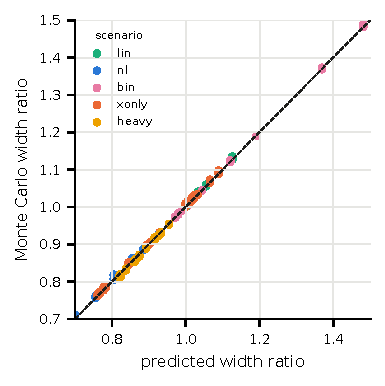
\includegraphics[width=\columnwidth]{figures/fig_theory.pdf}
  \caption{Predicted vs Monte Carlo width ratio for all oracle calibrators in \cref{tab:theory} and all $(n,N/n)$ cells. Dashed: identity.}
  \label{fig:theory}
\end{figure}

\section{Reproducibility checklist}
\label{app:checklist}

ICML 2026 does not require a separate checklist at submission (its call asks for supporting, reproducible evidence and a broader impact statement), but we give the relevant information here.

\begin{itemize}
  \item \textbf{Code and environment.} Python 3.11.2 with numpy 2.4.6, scipy 1.17.1, pandas 3.1.1, scikit-learn 1.9.1, ppi-python 0.2.3 (tag \texttt{v0.2.3}), gdown 6.5.1, matplotlib 3.11.2 (pinned in \texttt{requirements.txt}). Commands and runtime estimates are in \texttt{README.md}.
  \item \textbf{Data.} The nine \texttt{ppi-python} example pools, downloaded by the package loader; seven are used. No external data beyond these were used.
  \item \textbf{Seeds.} Every cell has a deterministic seed derived from its indices (see \texttt{README.md}).
  \item \textbf{Compute.} A 4-CPU quota. Total pipeline time \TOTALTIME{} (synthetic main about 100 min, real main about 165 min, pool and theory checks about 10 min).
  \item \textbf{Table and figure provenance.} \cref{tab:synth}: \texttt{run\_synth.py}, \texttt{summarize.py}, \texttt{make\_tables.py}. \cref{tab:real}, \cref{tab:realsens}, \cref{tab:pool}: \texttt{run\_real.py}, \texttt{theory\_pool.py}, \texttt{summarize.py}, \texttt{make\_tables.py}. \cref{tab:theory}, \cref{fig:theory}: \texttt{theory\_check.py}, \texttt{make\_tables.py}, \texttt{make\_figures.py}. \cref{fig:synth}: \texttt{make\_figures.py} (from \texttt{synth\_main\_summary.csv} and \texttt{theory\_check.csv}). \cref{fig:real}: \texttt{make\_figures.py} (from \texttt{real\_main.csv} and \texttt{theory\_pool.csv}). The large-$n$ extension: \texttt{run\_real.py --ns 5000 20000 --ratios 4} on four pools.
  \item \textbf{Failed or abandoned runs.} The first development run used a naive stratified-PPI variance and was discarded for that method (its rows are not used). The dev run for the learner choice used 100 replications per cell instead of 200 because of the CPU quota. No other runs were discarded.
\end{itemize}

\section{Literature check}
\label{app:lit}

References were checked against arXiv and publisher metadata pages. Starter references (PPI, PPI++, cross-PPI, active inference, StratPPI, DML) were read from their abstracts and, for StratPPI, from the full text to confirm the estimator form. For the three classical references (Zhang, Brown and Cai 2019; Chakrabortty and Cai 2018; Robins et al. 1994) we confirmed bibliographic metadata but not every claim in their full text, so we cite them only for the setting they treat. Incidental search results for unrelated semi-supervised papers were seen as snippets during this check; none was opened in full or used. We did not search for, open, or use any paper on shortening prediction-powered intervals under fixed labeled, unlabeled and predictor budgets beyond the starter list.


\end{document}
